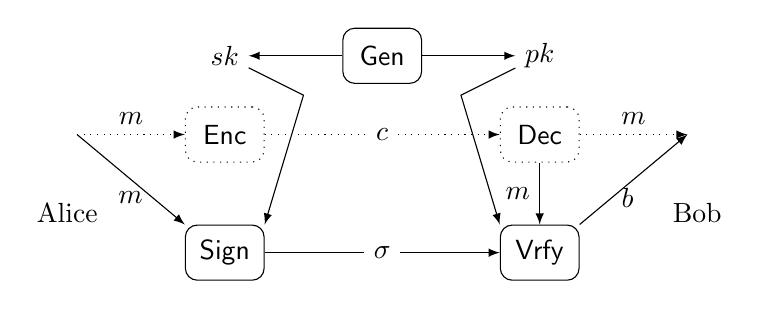
\begin{tikzpicture}[rc/.style={rounded corners=1ex, minimum width=1cm, minimum height=0.7cm}]
\node (sender) {\Alice};
\node (bart) [below of = sender] {Alice};
\node (enc) [draw, right of = sender, rc, dotted, node distance = 2cm] {$\mathsf{Enc}$};
\node (mac) [draw, below of = enc, rc, node distance = 1.5cm] {$\mathsf{Sign}$};
\node (k1) [above of = enc, node distance = 1cm] {$sk$};
\node (c) [right of = enc, node distance = 2cm] {$c$};
\node (t) [right of = mac, node distance = 2cm] {$\sigma$};
\node (gen) [draw, above of = c, rc,node distance = 1cm] {$\mathsf{Gen}$};
%\node (adv) [below of = c, node distance = 1cm] {\Adversary};
%\node (burns) [below of = adv] {Adversary};
\node (dec) [draw, right of = c, dotted,  rc,node distance = 2cm] {$\mathsf{Dec}$};
\node (ver) [draw, below of = dec, rc, node distance = 1.5cm] {$\mathsf{Vrfy}$};
\node (k2) [above of = dec, node distance = 1cm] {$pk$};
\node (receiver) [right of = dec, node distance = 2cm] {\Bob};
\node (lisa) [below of = receiver] {Bob};
\draw[ dotted, -latex] (sender) -- (enc) node [midway, above] {$m$};
\draw[ dotted] (enc) -- (c); \draw[ dotted, -latex] (c) -- (dec);
\draw (mac) -- (t); \draw[-latex] (t) -- (ver);
\draw[ dotted, -latex] (dec) -- (receiver) node [midway, above] {$m$};
%\draw[ dotted, -latex] (k1) -- (enc);
\draw[-latex] (gen) -- (k1);
\draw[-latex] (gen) -- (k2);								
%\draw[ dotted, -latex] (k2) -- (dec);
\draw[-latex] (sender.east) -- (mac.north west) node [pos=0.7, left] {$m$};	
\draw[-latex] (ver.north east) -- (receiver.west) node [pos=0.3, right] {$b$};
\draw[-latex] (dec) -- (ver) node [midway, left] {$m$};	
\draw[-latex] (k1) -- +(1cm,-0.5cm) -- (mac.north east);
\draw[-latex] (k2) -- +(-1cm,-0.5cm) -- (ver.north west);	
\end{tikzpicture}